\section{Results of the analysis}
\label{sec:results}
This chapter reports results in three steps: elicitation inputs and outputs, uncertainty propagation through \gls{upmavt}, and final rankings. Only results are reported here; interpretation and methodological implications are discussed in Section~\ref{sec:discussion}.

\subsection{Elicitation inputs and outputs}

\subsubsection{Full elicitation sessions}
The elicitation process involved four experts who performed all analytical steps: (1) quantitative indicator value function development, (2) qualitative indicator assessment and value function construction, and (3) weight determination using the \gls{pilebwt} methodology. Expert backgrounds are summarized in Table~\ref{tab:experts}, identities are maintained confidential.

\begin{table}[htbp]
	\centering
	\begin{tabularx}{\textwidth}{|c|X|X|}
		\hline
			extbf{Expert} & \textbf{Area of Expertise} & \textbf{Experience}\\
		\hline
		E1 & Risk Assessment (Academia) & Senior Scientist\\
		E2 & Nuclear Safety (Academia) & Senior Scientist\\
		E4 & Nuclear Safety (Industry) & Junior Engineer\\
		E8 & Energy System Modelling (Academia) & PhD Student\\
		\hline
	\end{tabularx}
	\caption{Experts involved in the elicitation process.}
	\label{tab:experts}
\end{table}

\subsubsection{Quick elicitation results}
\label{sec:quick_elicitation_results}
To enhance qualitative indicator characterization, five additional experts participated in an abbreviated "quick elicitation" process focused exclusively on qualitative indicators assessment (step 2). This expert panel is presented in Table~\ref{tab:quick_experts}.

\begin{table}[htbp]
	\centering
	\begin{tabular}{|c|c|c|}
		\hline
			extbf{Expert} & \textbf{Area of Expertise} & \textbf{Experience}\\
		\hline
		E3 & Nuclear Plants (Academia) & Academic Professor \\
		E5 & Project Controlling for Nuclear (Industry) & 20 years in Project Managment positions \\
		E6 & Nuclear new Construction (Industry) & 17 years in Nuclear Construction\\
		E7 & Nuclear Plant Managment (Industry / EU) & 17 years in Nuclear Operations, currently working for EU JRC\\
		E9 & Probability Safety Assessment (Industry / UN)& 15 years in PSA for Nuclear related projects, currently working at IAEA\\
		\hline
	\end{tabular}
	\caption{Experts involved in the quick elicitation process.}
	\label{tab:quick_experts}
\end{table}

Figure~\ref{fig:quick_examples} illustrates the results for "Design Complexity", presented as a value heatmap to visualize the elcited values to each alternative across all experts.

\begin{figure}[htbp]
	\centering
	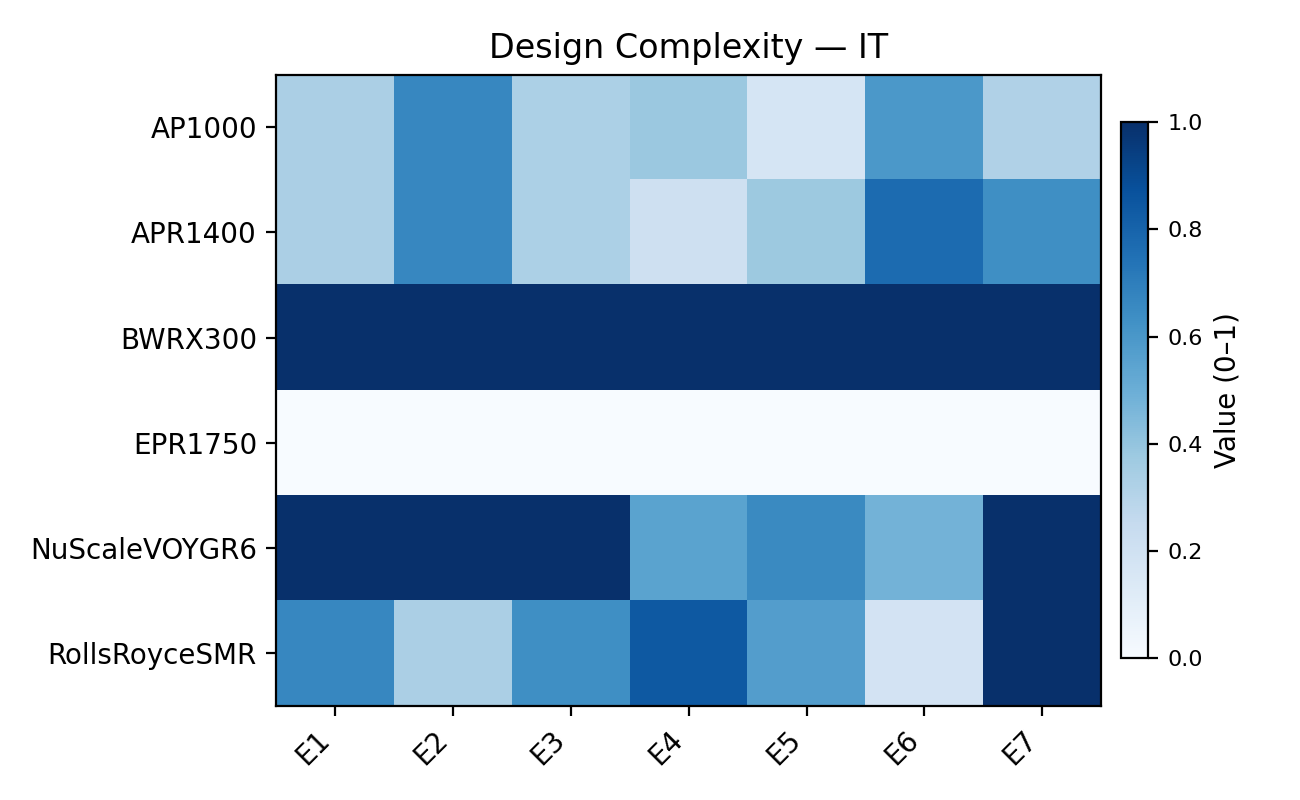
\includegraphics[width=0.75\linewidth]{imgs/QI_result_example.png}
	\caption{Values for the qualitative indicator "Design Complexity".}
	\label{fig:quick_examples}
\end{figure}

\subsubsection{Representative elicitation outputs}
Figure~\ref{fig:vf_examples} presents the value functions elicited from the four experts for the same indicator, showing the divergencies between expert opinions. Figure~\ref{fig:weight_space_results} shows weight elicitation outcomes presenting the feasible weight space, explored via differential evolution (SciPy implementation \cite{PLACEHOLDER}). Figure~\ref{fig:consistency_results} presents the consistency plots, which compare the declared pairwise comparison ratios with the ratios between the optimized weights. Each second bar represents the mean weight sampled from the feasible solution space, with error bars indicating $\pm \sigma$ to quantify solution variability. This adapted presentation, building on \cite{PLACEHOLDER}'s consistency analysis, explicitly incorporates uncertainty bounds from the weight space exploration.

\begin{figure}[htbp]
	\centering
	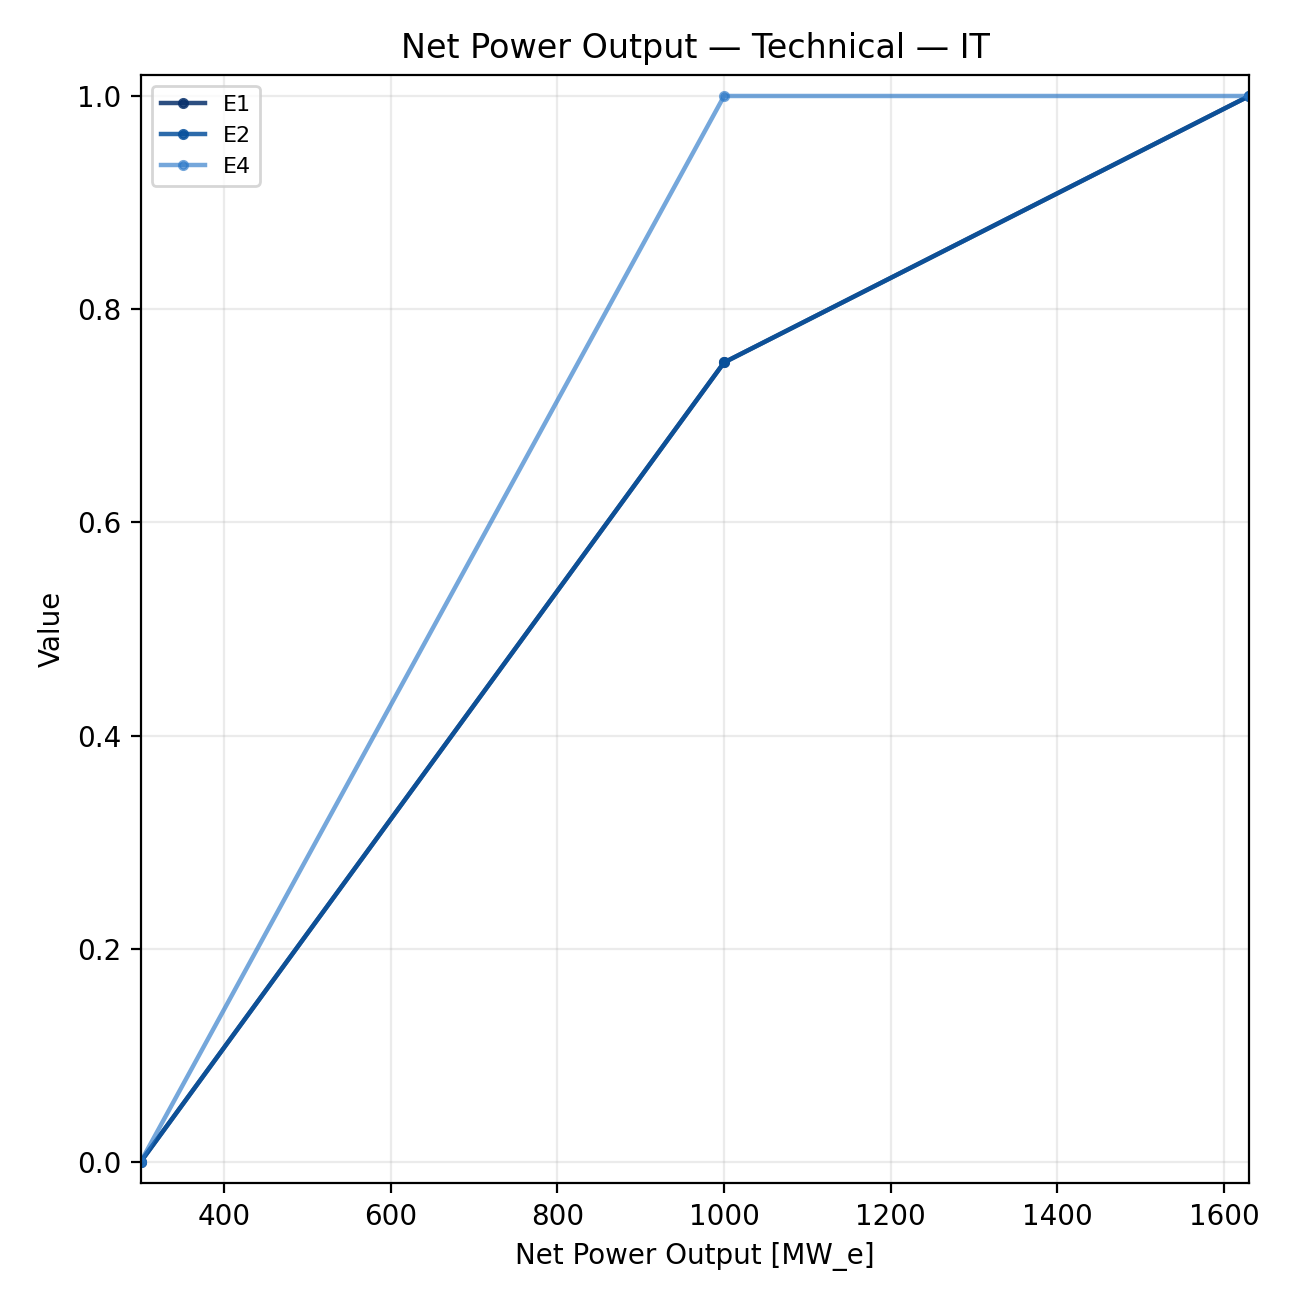
\includegraphics[width=0.5\linewidth]{imgs/vf_result_example.png}
	\caption{Value function elicited by experts for "Net Power Output - IT".}
	\label{fig:vf_examples}
\end{figure}

\begin{figure}[htbp]
	\centering
	
\includegraphics[width=0.95\linewidth]{weight_space_example.pdf}
	\caption{Weight plot space for expert E4.}
	\label{fig:weight_space_results}
\end{figure}

\begin{figure}[p]
	\centering
	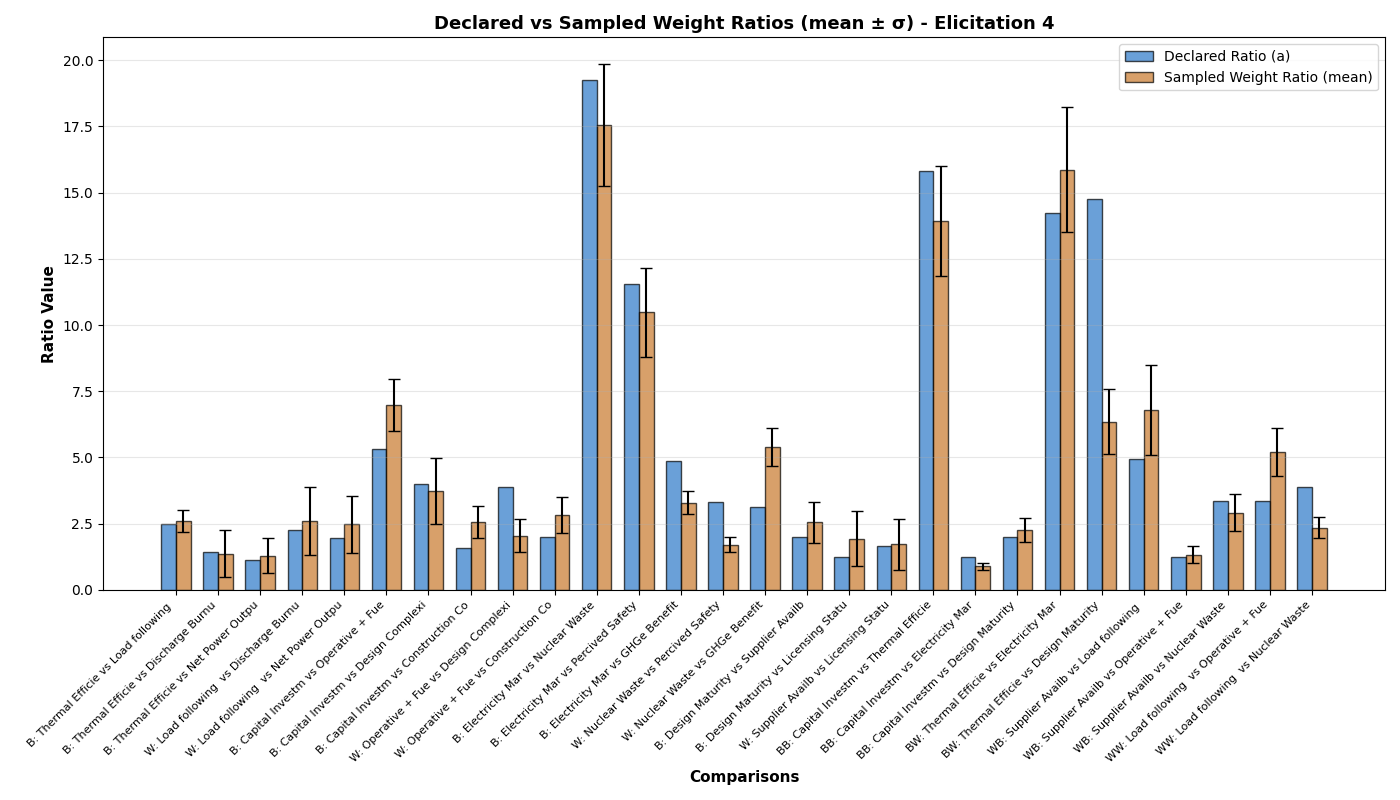
\includegraphics[angle=90,height=\textheight,keepaspectratio]{imgs/consistency_plot_example.png}
	\caption{Consistency plot for expert E4.}
	\label{fig:consistency_results}
\end{figure}

\subsection{UP-MAVT}
As established in Section~\ref{sec:uncertanty_propagation_mcda}, the \gls{smc} and \gls{nsmc} approaches serve complementary purposes. \gls{smc} results evaluate pre-aggregation uncertainty and expert consensus levels, while \gls{nsmc} generates final rankings. Representative outputs for one of the countries are presented in Figure~\ref{fig:smc_france_sum}, comparing weighted sum aggregation methodology.

\begin{figure}[htbp]
	\centering
	
\includegraphics[width=0.95\linewidth]{Phase2_WeightedSum_Strict_FR_20260127_170138_histograms.pdf}
	\caption{\gls{smc} results for France using weighted sum aggregation (2000 iterations per expert).}
	\label{fig:smc_france_sum}
\end{figure}

\begin{figure}[htbp]
	\centering
	
\includegraphics[width=0.95\linewidth]{Phase2_Geometric_Strict_FR_20260128_092214_histograms.pdf}
	\caption{\gls{smc} results for France using geometric mean aggregation, showing broader distributions and reduced dominance patterns.}
	\label{fig:smc_france_geo}
\end{figure}

\subsection{Rankings}
Ranking heatmaps are reported for each country across the three aggregation methods. Figures~\ref{fig:aggregation_methods_comparison_france}--\ref{fig:nsmc_rankings_po} present the \gls{nsmc} results using geometric mean aggregation for the country-specific summaries, alongside a cross-method comparison for France.

\begin{figure}[htbp]
    \centering
    \subfloat[\gls{sum}]{
\includegraphics[width=0.32\linewidth]{Phase3_AllMethods_FR_weighted_sum_20260127_171441_heatmap.pdf}}\hfill
    \subfloat[\gls{geo}]{
\includegraphics[width=0.32\linewidth]{Phase3_AllMethods_FR_geometric_mean_20260127_171648_heatmap.pdf}}\hfill
    \subfloat[\gls{har}]{
\includegraphics[width=0.32\linewidth]{Phase3_AllMethods_FR_harmonic_mean_20260127_171543_heatmap.pdf}}
    \caption{France: \gls{nsmc} ranking heatmaps obtained with different aggregation methods. Results show dominance of large reactor designs and ranking sensitivity to compensation method.}
    \label{fig:aggregation_methods_comparison_france}
\end{figure}

\begin{figure}[htbp]
    \centering
    
\includegraphics[width=0.95\linewidth]{Phase3_AllMethods_IT_geometric_mean_20260127_171336_heatmap.pdf}
    \caption{Italy: \gls{nsmc} ranking heatmap with geometric mean aggregation.}
    \label{fig:nsmc_rankings_it}
\end{figure}

\begin{figure}[htbp]
    \centering
    
\includegraphics[width=0.95\linewidth]{Phase3_AllMethods_CH_geometric_mean_20260127_172000_heatmap.pdf}
    \caption{Switzerland: \gls{nsmc} ranking heatmap with geometric mean aggregation.}
    \label{fig:nsmc_rankings_ch}
\end{figure}

\begin{figure}[htbp]
    \centering
    
\includegraphics[width=0.95\linewidth]{Phase3_AllMethods_PO_geometric_mean_20260127_172306_heatmap.pdf}
    \caption{Poland: \gls{nsmc} ranking heatmap with geometric mean aggregation.}
    \label{fig:nsmc_rankings_po}
\end{figure}

